\subsection{Pruebas Ejecutadas.}
En la siguiente captura de pantalla se muestran los par\'{a}metros del la caja de b\'{u}squeda
empleados en las pruebas realizadas con Scoops3D.\\

\begin{figure}[H]
\centering
	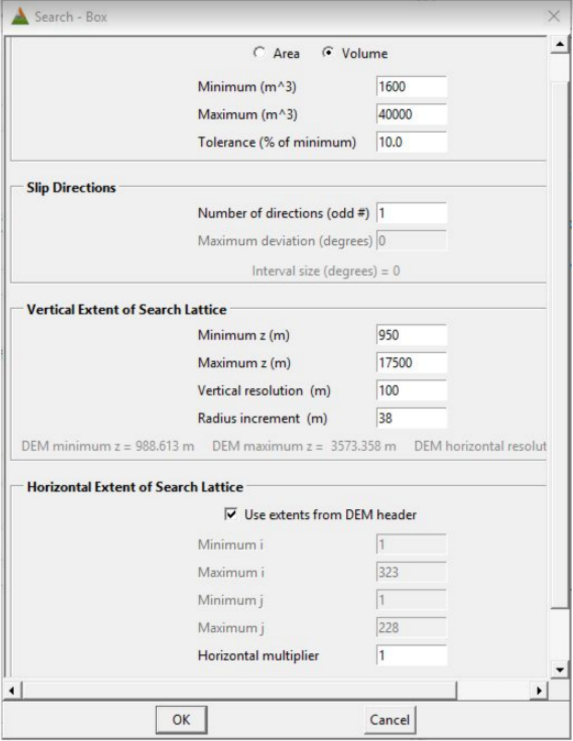
\includegraphics[scale=0.6]{search_setup.PNG} 
	\caption{Par\'ametros usados en la ejecuci\'on de pruebas preliminares.}

\end{figure}


Se trabaj\'{o} con el rango de b\'{u}squeda de movimientos en masa por rango de volumen,
basado en los movimientos registrados en la base de datos SIMA para la zona de trabajo.
Para cada nodo de b\'{u}squeda se analiza solamente una direcci\'{o}n de deslizamiento.
En la extensi\'{o}n vertical de las dovelas de falla se toma una altura ligeramente inferior a la
altura menor existente en el DEM y como altura m\'{a}xima se tom\'{o} una altura de 17500
msnm,esta \'{u}ltima se determin\'{o} luego de m\'{u}ltiples pruebas variando la altura m\'{a}xima hasta
que se pudo apreciar que no se detectaban nuevas superficies de falla(de \'area significativa) al continuar
aumentando la altura m\'{a}xima del nodo central, para lo cual se us\'{o} el archivo Boundcheck, de acuerdo con las recomendaciones contenidas en el manual de Scoops3D. Una ilustraci\'on del archivo Boundcheck de la prueba realizada con par\'ametros de resistencia menos competentes se muestra en la figura \ref{fig:boundcheck} 

\begin{figure}[H]
\centering
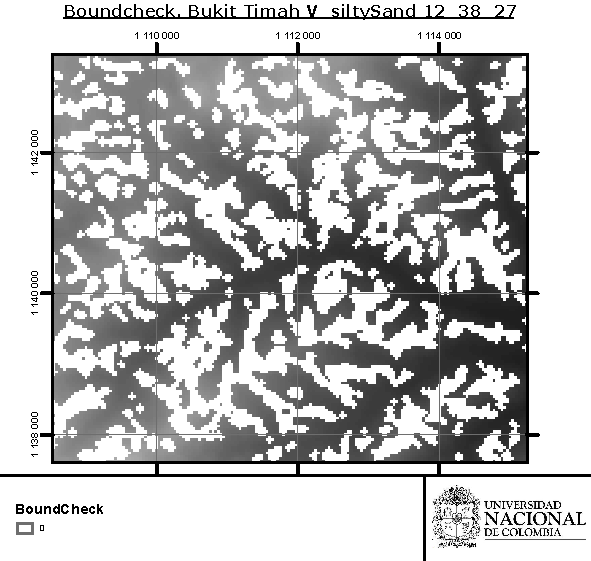
\includegraphics[scale=1]{img/boundcheck.pdf}
\caption{Mapa de distribuciones del factor Boundcheck mencionado en la recci\'n \ref{chap: archivos de salida}.
N\'otese que en su totalidad, el archivo raster Boundcheck est\'a compuesto por valores 0 (blanco) y -9999 (transparente) }
\label{fig:boundcheck}
\end{figure}




\begin{wrapfigure}{l}{0.1\textwidth} %this figure will be at the right
    \centering
    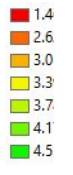
\includegraphics[scale=0.7]{symbology.PNG}
\end{wrapfigure}


Se ha implementado una escala de calor para los valores de factor de seguridad a los
pixeles de los archivos fos3D\textunderscore out.asc, aunque se han obtenido factores de seguridad hasta
un valor de 100, a los p\'ixeles con valor superior a 5 se les ha asignado la misma tonalidad
de verde.
\\

